%%%%%%%%%%%%%%%%%%%%%%%%%%%%%%%%%%%%%%%%%
% Wenneker Article
% LaTeX Template
% Version 2.0 (28/2/17)
%
% This template was downloaded from:
% http://www.LaTeXTemplates.com
%
% Authors:
% Vel (vel@LaTeXTemplates.com)
% Frits Wenneker
%
% License:
% CC BY-NC-SA 3.0 (http://creativecommons.org/licenses/by-nc-sa/3.0/)
%
%%%%%%%%%%%%%%%%%%%%%%%%%%%%%%%%%%%%%%%%%

%----------------------------------------------------------------------------------------
%	PACKAGES AND OTHER DOCUMENT CONFIGURATIONS
%----------------------------------------------------------------------------------------

\documentclass[10pt, a4paper, twocolumn]{article} % 10pt font size (11 and 12 also possible), A4 paper (letterpaper for US letter) and two column layout (remove for one column)

\usepackage[english]{babel} % English language hyphenation
\usepackage{microtype} % Better typography
\usepackage{amsmath,amsfonts,amsthm} % Math packages for equations
\usepackage[svgnames]{xcolor} % Enabling colors by their 'svgnames'
\usepackage[hang, small, labelfont=bf, up, textfont=it]{caption} % Custom captions under/above tables and figures
\usepackage{booktabs} % Horizontal rules in tables
\usepackage{lastpage} % Used to determine the number of pages in the document (for "Page X of Total")
\usepackage{graphicx} % Required for adding images
\usepackage{amssymb}
\usepackage[mathscr]{eucal}
\usepackage[table]{xcolor}
\usepackage{enumitem} % Required for customising lists
\setlist{noitemsep} % Remove spacing between bullet/numbered list elements
\usepackage{sectsty} % Enables custom section titles
\allsectionsfont{\usefont{OT1}{phv}{b}{n}} % Change the font of all section commands (Helvetica)
\usepackage{hyperref}
\usepackage[sort,numbers]{natbib}
%----------------------------------------------------------------------------------------
%	MARGINS AND SPACING
%----------------------------------------------------------------------------------------
\usepackage{geometry} % Required for adjusting page dimensions
\geometry{
	top=0.65cm, % Top margin
	bottom=1.5cm, % Bottom margin
	left=1.5cm, % Left margin
	right=1.5cm, % Right margin
	includehead, % Include space for a header
	includefoot, % Include space for a footer
	%showframe, % Uncomment to show how the type block is set on the page
}
\setlength{\columnsep}{6mm} % Column separation width


%----------------------------------------------------------------------------------------
%	FONTS
%----------------------------------------------------------------------------------------

\usepackage[T1]{fontenc} % Output font encoding for international characters
\usepackage[utf8]{inputenc} % Required for inputting international characters
\usepackage{XCharter} % Use the XCharter font

%%%%%%%%%%%%%%%%%%%%%%%%%%%%%%%%%%%%%%%%%%
% Wenneker Article
% Structure Specification File
% Version 1.0 (28/2/17)
%
% This file originates from:
% http://www.LaTeXTemplates.com
%
% Authors:
% Frits Wenneker
% Vel (vel@LaTeXTemplates.com)
%
% License:
% CC BY-NC-SA 3.0 (http://creativecommons.org/licenses/by-nc-sa/3.0/)
%
%%%%%%%%%%%%%%%%%%%%%%%%%%%%%%%%%%%%%%%%%

%----------------------------------------------------------------------------------------
%	PACKAGES AND OTHER DOCUMENT CONFIGURATIONS
%----------------------------------------------------------------------------------------

\usepackage[english]{babel} % English language hyphenation

\usepackage{microtype} % Better typography

\usepackage{amsmath,amsfonts,amsthm} % Math packages for equations

\usepackage[svgnames]{xcolor} % Enabling colors by their 'svgnames'

\usepackage[hang, small, labelfont=bf, up, textfont=it]{caption} % Custom captions under/above tables and figures

\usepackage{booktabs} % Horizontal rules in tables

\usepackage{lastpage} % Used to determine the number of pages in the document (for "Page X of Total")

\usepackage{graphicx} % Required for adding images

\usepackage{enumitem} % Required for customising lists
\setlist{noitemsep} % Remove spacing between bullet/numbered list elements

\usepackage{sectsty} % Enables custom section titles
\allsectionsfont{\usefont{OT1}{phv}{b}{n}} % Change the font of all section commands (Helvetica)

%----------------------------------------------------------------------------------------
%	MARGINS AND SPACING
%----------------------------------------------------------------------------------------

\usepackage{geometry} % Required for adjusting page dimensions

\geometry{
	top=1cm, % Top margin
	bottom=1.5cm, % Bottom margin
	left=2cm, % Left margin
	right=2cm, % Right margin
	includehead, % Include space for a header
	includefoot, % Include space for a footer
	%showframe, % Uncomment to show how the type block is set on the page
}

\setlength{\columnsep}{7mm} % Column separation width

%----------------------------------------------------------------------------------------
%	FONTS
%----------------------------------------------------------------------------------------

\usepackage[T1]{fontenc} % Output font encoding for international characters
\usepackage[utf8]{inputenc} % Required for inputting international characters

\usepackage{XCharter} % Use the XCharter font

%----------------------------------------------------------------------------------------
%	HEADERS AND FOOTERS
%----------------------------------------------------------------------------------------

\usepackage{fancyhdr} % Needed to define custom headers/footers
\pagestyle{fancy} % Enables the custom headers/footers

\renewcommand{\headrulewidth}{0.0pt} % No header rule
\renewcommand{\footrulewidth}{0.4pt} % Thin footer rule

\renewcommand{\sectionmark}[1]{\markboth{#1}{}} % Removes the section number from the header when \leftmark is used

%\nouppercase\leftmark % Add this to one of the lines below if you want a section title in the header/footer

% Headers
\lhead{} % Left header
\chead{\textit{\thetitle}} % Center header - currently printing the article title
\rhead{} % Right header

% Footers
\lfoot{} % Left footer
\cfoot{} % Center footer
\rfoot{\footnotesize Page \thepage\ of \pageref{LastPage}} % Right footer, "Page 1 of 2"

\fancypagestyle{firstpage}{ % Page style for the first page with the title
	\fancyhf{}
	\renewcommand{\footrulewidth}{0pt} % Suppress footer rule
}

%----------------------------------------------------------------------------------------
%	TITLE SECTION
%----------------------------------------------------------------------------------------

\newcommand{\authorstyle}[1]{{\large\usefont{OT1}{phv}{b}{n}\color{DarkRed}#1}} % Authors style (Helvetica)

\newcommand{\institution}[1]{{\footnotesize\usefont{OT1}{phv}{m}{sl}\color{Black}#1}} % Institutions style (Helvetica)

\usepackage{titling} % Allows custom title configuration

\newcommand{\HorRule}{\color{DarkGoldenrod}\rule{\linewidth}{1pt}} % Defines the gold horizontal rule around the title

\pretitle{
	\vspace{-30pt} % Move the entire title section up
	\HorRule\vspace{10pt} % Horizontal rule before the title
	\fontsize{32}{36}\usefont{OT1}{phv}{b}{n}\selectfont % Helvetica
	\color{DarkRed} % Text colour for the title and author(s)
}

\posttitle{\par\vskip 15pt} % Whitespace under the title

\preauthor{} % Anything that will appear before \author is printed

\postauthor{ % Anything that will appear after \author is printed
	\vspace{10pt} % Space before the rule
	\par\HorRule % Horizontal rule after the title
	\vspace{20pt} % Space after the title section
}

%----------------------------------------------------------------------------------------
%	ABSTRACT
%----------------------------------------------------------------------------------------

\usepackage{lettrine} % Package to accentuate the first letter of the text (lettrine)
\usepackage{fix-cm}	% Fixes the height of the lettrine

\newcommand{\initial}[1]{ % Defines the command and style for the lettrine
	\lettrine[lines=3,findent=4pt,nindent=0pt]{% Lettrine takes up 3 lines, the text to the right of it is indented 4pt and further indenting of lines 2+ is stopped
		\color{DarkGoldenrod}% Lettrine colour
		{#1}% The letter
	}{}%
}

\usepackage{xstring} % Required for string manipulation

\newcommand{\lettrineabstract}[1]{
	\StrLeft{#1}{1}[\firstletter] % Capture the first letter of the abstract for the lettrine
	\initial{\firstletter}\textbf{\StrGobbleLeft{#1}{1}} % Print the abstract with the first letter as a lettrine and the rest in bold
}

%----------------------------------------------------------------------------------------
%	BIBLIOGRAPHY
%----------------------------------------------------------------------------------------

\usepackage[backend=bibtex,style=authoryear,natbib=true]{biblatex} % Use the bibtex backend with the authoryear citation style (which resembles APA)

\addbibresource{example.bib} % The filename of the bibliography

\usepackage[autostyle=true]{csquotes} % Required to generate language-dependent quotes in the bibliography
 % Specifies the document structure and loads requires packages

%----------------------------------------------------------------------------------------
%	ARTICLE INFORMATION
%----------------------------------------------------------------------------------------
\begin{document}



\title{$\mathcal{ROBHOOT}$ \\ Open Research Network \\ Whitepaper v.2.0} % The article title
  \author{Universal Neutrality team{\textsuperscript{1,2,3} and XY\textsuperscript{2,3}} % Authors
  \newline\newline % Space before institutions
  \\
	\textsuperscript{1}\institution{}\\ % Institution 1
	\textsuperscript{2}\institution{}\\ % Institution 2
	%\textsuperscript{3}\institution{\texttt{LaTeXTemplates.com}}
      %} % Institution 3


% Example of a one line author/institution relationship
%\author{\newauthor{John Marston} \newinstitution{Universidad Nacional Autónoma de México, Mexico City, Mexico}}

\date{\today} % Add a date here if you would like one to appear underneath the title block, use \today for the current date, leave empty for no date
%---------------------------------------------------------------------------------------

%\begin{document}

\maketitle % Print the title
\thispagestyle{firstpage} % Apply the page style for the first page (no headers and footers)

%----------------------------------------------------------------------------------------
%	ABSTRACT
%----------------------------------------------------------------------------------------
\lettrineabstract{\section{{\bf Summary}}

  Global sustainability is a major goal of humanity. Many studies have
  shown global sustainability could be achieved by strengthening
  transparency and feedbacks between social, ecological and governance
  systems. Sustainability goals, however, strongly depend on global
  society access to evidence- and research-based knowledge gaps. Yet,
  the science ecosystem lack open-source technologies narrowing down
  knowledge gaps. Here, we introduce an open research network
  targeting a reduction of knowledge gaps by generating open-access,
  immutable and reproducible global science reports. Such features
  encompass a hybrid-automated-technology to lay out the foundation of
  an open-science ecosytem strengthening the robustness,
  decentralization, reproducibility and social accessibility of
  science. The project summarized here is not set out to deliver a
  finished research open network, but to provide the architecture of a
  science-enabled technology as a prototype proof-of-principle to
  connect decentralized and neutral-knowledge generation with
  knowledge-inspired societies.}

 
%----------------------------------------------------------------------------------------
%	ARTICLE CONTENTS
%----------------------------------------------------------------------------------------
\section{The Science Ecosystem}
Science and technology contain multiple steps of information transfer
among trusted/untrusted peers. As a consequence, science generates
knowledge with specific features. Which are the desirable features of
human-generated knowledge? Should such desirable features be aligned
with taking informed decisions in complex social, governance,
environmental and technological problems? How much global transparency
in knowledge generation can be achieved to facilitate sustainability
goals of humanity? Currently public funded science is highly
centralized \citep{Inhaber1977,Gunther2018}⁠⁠, prone to errors
\citep{Fang2011}, difficult to reproduce \citep{Hardwicke2018}, and
contains many biases \citep{Ioannidis2005}. This makes science an
ecosystem with increasing problems to decrease the evidence- and
research-based knowledge gaps in humanity
\citep{Mastrangelo2019}. Here we propose an open research network
fully accounting for the research cycle. The goal of such a technology
is to reduce global knowledge gaps while accounting for
centralization, bias, error-prone, non-reproducibility and lack of
incentives in the existing science and technology ecosystem (Figure 1
and Table 1).
%\vspace{0.15 in}
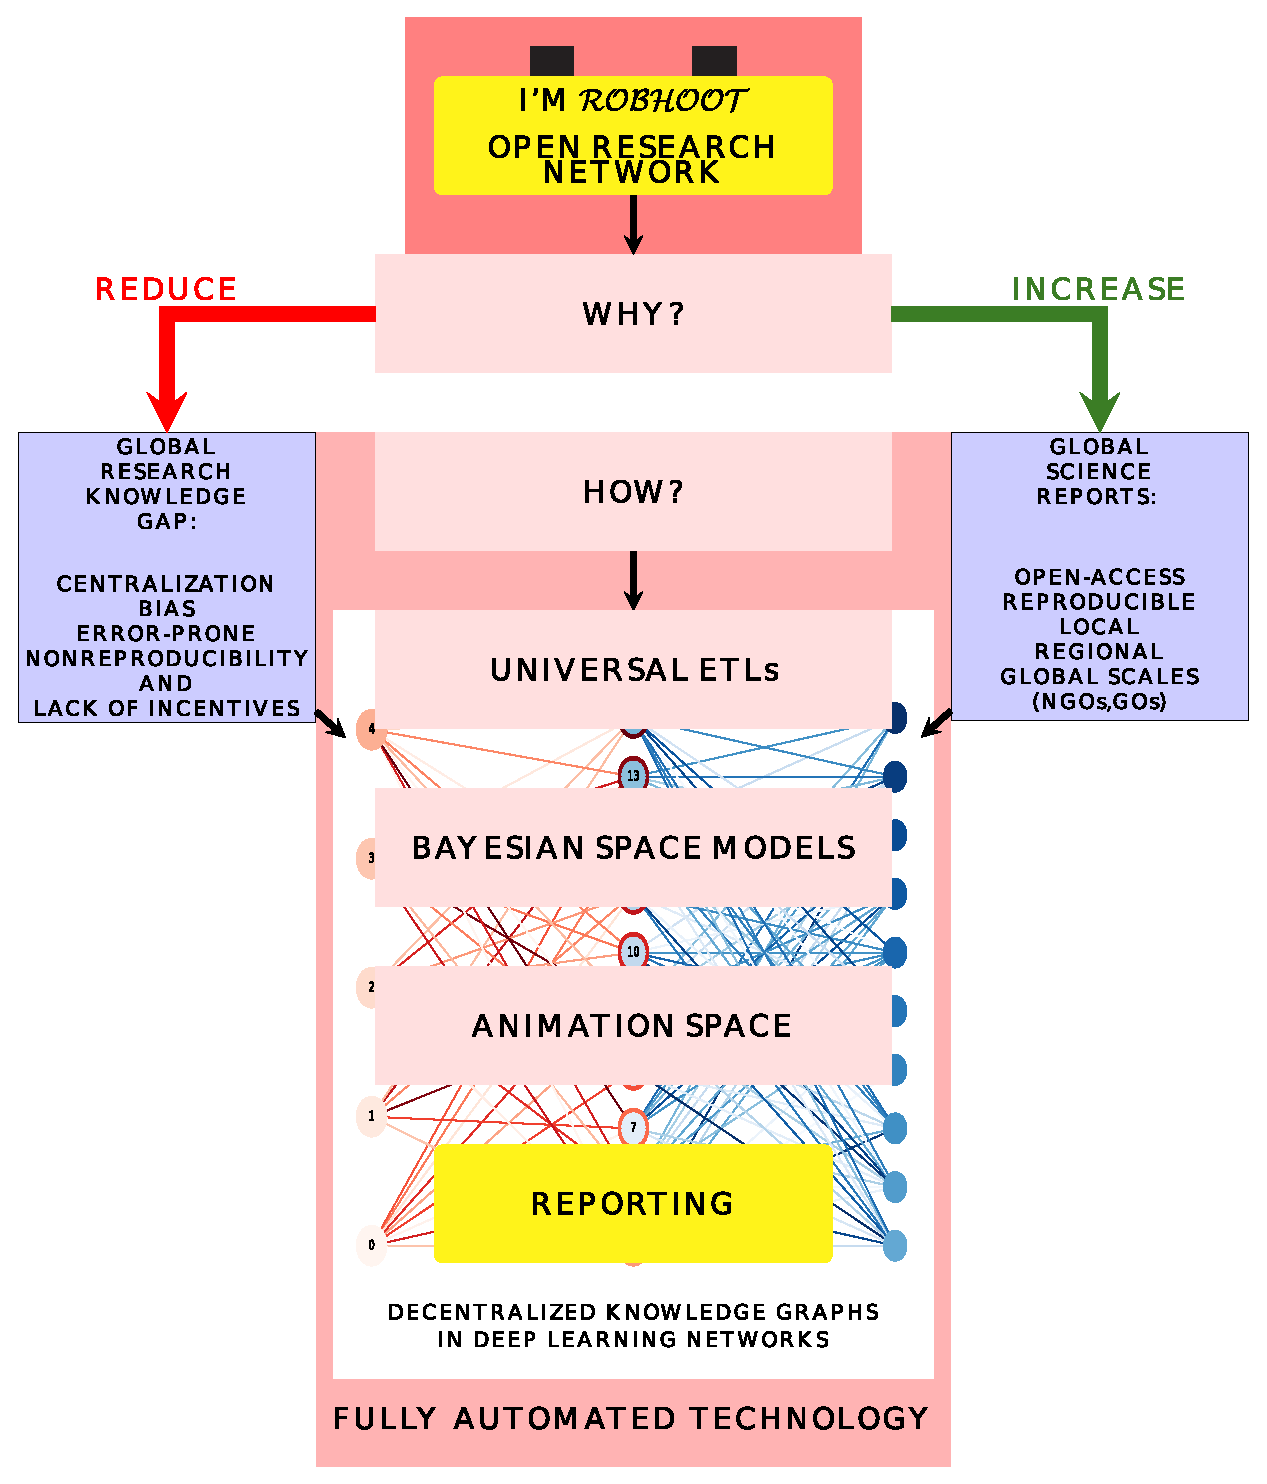
\includegraphics[width=0.45\textwidth]{flowchart.pdf}

{\small {\bf Figure 1: Open research network technology}. {\bf
    $\mathcal{ROBHOOT}$} targets a decrease of global knowledge gaps
  by reducing key features of science (red path) while increasing
  reproducible and global open-access reports (green path). The
  following is an scheme for an open-source science-based technology
  in the digital ecosystem: First, {\bf Universal ETLs} (i.e.,
  Extraction, Transformation and Load algorithms) to formalize
  database integration and complexity reduction. {\bf Bayesian Space
    Models} accounting for open-ended optimization techniques. Third,
  {\bf Animation Space} visualizing fitting procedures and pattern
  generation connecting empirical data and models. Four, {\bf
    Reporting} in natural processing language based on knowledge
  graphs, and fifth, {\bf Decentralized Deep Learning Methods} to
  automate knowledge graph generation making them immutable, open and
  globally accessible.}
The core feature of an open research network is to embed
knowledge-generation into reproducible automation and
decentralization. Currently, many studies focusing on decentralized
ecosystems are producing an immense gain of knowledge in a variety of
sectors about scalability, security and decentralization trade-offs
\citep{Golem2016,Durov2017,Androulaki2018,OceanProtocolFoundation2018,BigchainDBGmbH2018}. In
the open science ecosystem, only a few implementations of
decentralized technologies exist \citep{Gunther2018}. Automation and
AI technologies represent the other angle from which many advances are
rapidly occurring in digital ecosystems
\citep{Schmidhuber:2015,Reichstein,Gil2019}. While the existing
technological paradigm in many sectors is rapidly shifting towards
science-based decentralization and automation technologies, the
science ecosystem currently lack decentralized, neutral and
open-source knowledge-inspired technologies strongly impacting
knowledge-inspired societies (Figure 1 and Table 1). Rapid advances of
research platforms automating parts of the research cycle are
currently under development Automating
\citep{Steinruecken,Guimera}.\footnote{This is by no means an
  exhaustive list but it gives an indication of the many projects
  currently in place:
  \href{https://www.nterminal.com}{NakamotoT},\href{https://cloud.google.com/bigquery/}{BigQuery},\href{https://www.automaticstatistician.com/index/}{Automated
    statistician},\href{http://www.modulos.ai/}{Modulos},\href{https://ai.google/}{Google
    AI},\href{https://iris.ai}{Iris},\href{https://github.com/DS3Lab/easeml}{easeml}\href{https://www.datarobot.com/}{datarobot}\href{https://aito.ai/}{aito}}
Most of the existing research projects aiming to automate part of the
research cycle are being built around close-source
software. Therefore, open-source, reproducible, decentralized and
automated technologies accounting for the research cycle are at a very
incipient stage of development. To move forward open-source
technologies accounting for the research cycle we need to compactly
integrate knowledge-generation (Figure 2a) to automated tools
connecting knowledge graphs (Figure 2b) and deep learning networks
(Figure 2c) in fully decentralized ecosystems (Figure 2d).
\begin{table}
 %\rowcolor{pink}
\begin{tabular}{ p{3cm} | p{2cm} | p{2cm}}
  \hline \hline
  \textbf{Features} & \textbf{Science Ecosystem} &\textbf{{\bf $\mathcal{ROBHOOT}$}}\\  \hline
  Decentralization & No & Yes \\ \hline
  Full automation & No & Yes \\ \hline
  Open-access & Mostly No & Yes \\ \hline
  Immutability & No & Yes \\ \hline
  Robustness & Mostly No & Yes \\ \hline
  Reproducibility & Mostly No & Yes \\ \hline        
  Owner-Controlled assets & No & Yes \\ \hline       
  \bottomrule
\end{tabular}
\caption{{\bf $\mathcal{ROBHOOT}$} is designed to resolve desirable
  properties of science: Open-access, immutability, robustness,
  reproducibility, and owner-controlled assets. These features will be
  added during the different stages of development of the project
  (section ``Design Goals'').}
\end{table}
% ------------------------------------------------
  \section{Design Goals}
  The open research network will be developed in four stages. The most
  advanced version is to provide real-time open-access reporting in a
  decentralized network (Table 2). Figures 1 to 4 show goals and
  architecture, milestones, the digital ecosystem and the timeline for
  each of the stages, respectively.
  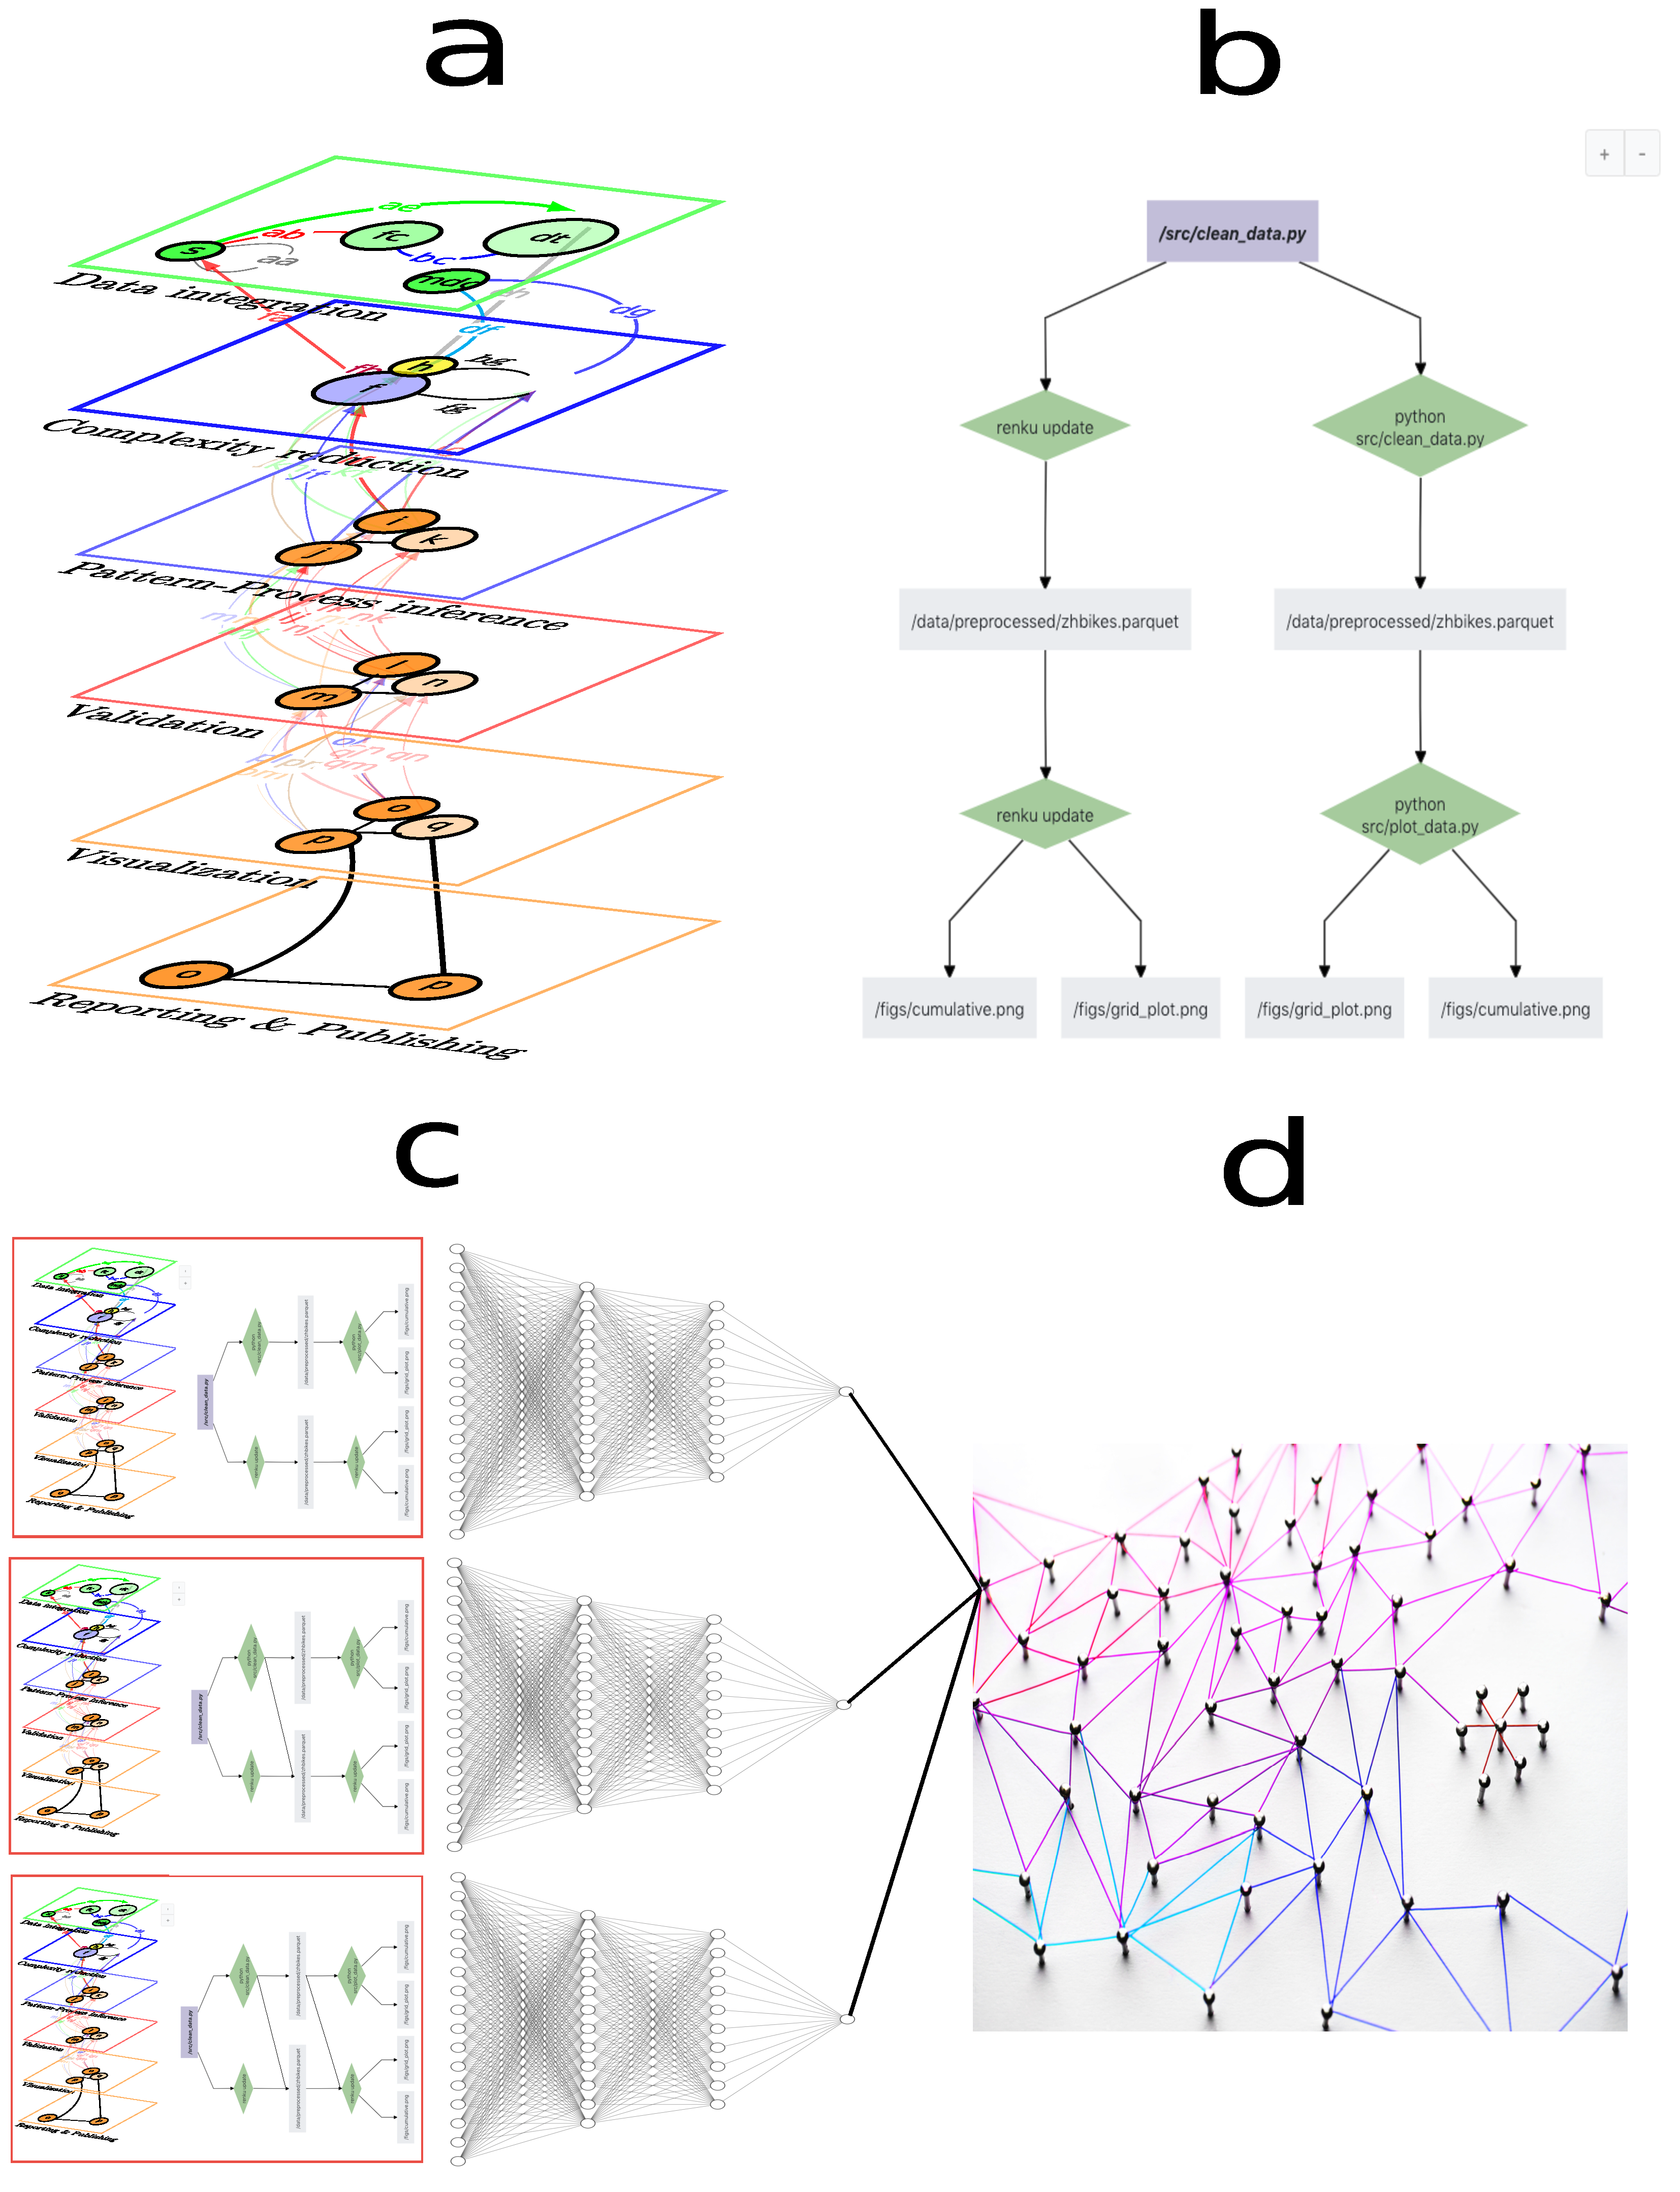
\includegraphics[width=0.45\textwidth]{Figure1.pdf}
  % \begin{figure*}[ht]
  
  {\small {\bf Figure 2: Milestones}. {\bf a}) {\bf
      $\mathcal{ROBHOOT}$ v.1.0} features a fully automated research
    cycle from data integration to reporting generation. {\bf b}) {\bf
      $\mathcal{ROBHOOT}$ v.2.0} traces research paths as shown in
    {\bf a} using knowledge graphs (KGs). {\bf c}) {\bf
      $\mathcal{ROBHOOT}$ v.3.0} contrasts deep leaning networks to
    explore populations of KGs for gaining undestanding of the
    process-based patterns contained in the data, and {\bf d}) {\bf
      $\mathcal{ROBHOOT}$ v.4.0} deploys KGs in a decentralized
    network of trusting/untrusting peers with every peer maintaining
    the population of the KGs.}
  %\end{figure*}
  
  The overall objectives including tools, methods, and territory to
  explore in each stage for each of the four major versions are the
  following:
  %\vspace{-0.15 in}
  \subsection{{\bf $\mathcal{ROBHOOT}$ v.1.0}: \\Automated Research Cycle}
   \begin{itemize}
   \item {\bf Universal ETLs} connects open-source generalized
     fault-tolerance algorithms to extract, transform and load data
     with unique features (i.e., formats, historical-real time,
     storage, dimensions, size, sampling bias and spatiotemporal
     resolution, etc) (Figures 1 and 2a, two top layers).
   \item {\bf Bayesian space models} explore open-ended language of
     models combining Bayesian networks and optimization methods. The
     Bayesian space models module will search, evaluate models,
     trading-off complexity, fit to data and quantify resource usage
     (Figures 1 and 2a, inference and validation layers). 
   \item {\bf Animation Space} will connect open-source visualization
     software to the exploration of open-ended models to make the
     whole search transparent, highly visual and reproducible (Figures
     1 and 2a, visualization layer).
   \item {\bf Reporting} will develop a procedure to automatically
     explain the structure of the Bayesian space modeling module. It
     will also communicate the module using visualizations of the
     procedures followed by the Universal ETLs and Bayesian space
     models modules (Figures 1 and 2a, reporting layer).
   \item Robhoot 1.0 testnet will produce global automated reports on
     ``Biodiversity, Global Change and Sustainability Research'' to
     explore the robustness of the automated research cycle accounting
     for {\bf Universal ETLs}, {\bf Bayesian space models}, {\bf
       Animation space} algorithms and {\bf Reporting} in natural
     processing languages.
   \end{itemize}

   \begin{itemize}
   \item {\bf Tools and Methods}: Multilayer networks metrics,
     Bayesian Networks, Julia, Python, Open-source software protocols,
     Gitchain, ETLs open-source software, Kafka, Clickhouse, Fluentd,
     Hadoop.
   \end{itemize}

    \begin{itemize}
    \item {\bf Novel territory}: Develop universal open-source ETLs
      algorithms and Bayesian space models and connect them to
      reporting automation in a ``Biodiversity, Global Change and
      Sustainability Research'' case study.
   \end{itemize}

   
 %\vspace{-0.15 in}
   
  \subsection{{\bf $\mathcal{ROBHOOT}$ v.2.0}: \\ Knowledge Graphs}
  \begin{itemize}
  \item Implementation of algorithms tracking paths of the research
    cycle with Knowledge Graphs (KGs) (Figure 2b).
  \item Robustness and stability of searching and fitting procedures
    following a suite of open-source lineage client-tracker
    algorithms.
  \end{itemize}

   \begin{itemize}
   \item {\bf Tools and Methods}: Knowlegde graph algorithms and
     open-source packages (i.e., Renku and others).
   \end{itemize}

    \begin{itemize}
    \item {\bf Novel Territory}: Contrasting a set of Knowledge Graphs
      algorithms to explore the reproducibility properties of the full
      research cycle.
   \end{itemize}

  %\vspace{-0.15 in}
  
  \subsection{{\bf $\mathcal{ROBHOOT}$ v.3.0}: \\ Deep learning networks}
  \begin{itemize}
  \item Deployment of deep learning algorithms to sample paths of the
    research cycle to produce populations of Knowledge Graphs (KGs)
    (Figures 2a-c).
  \item Exploration of the robustness of the automated research cycle
    combining optimization algorithms and the population of Knowledge
    Graphs (Figure 2c).
  \end{itemize}

 \begin{itemize}
 \item {\bf Tools and Methods}: Neural Biological Networks, Spiking
   networks, Bayesian Networks, Deep learning networks. Optimization
   algorithms.
 \end{itemize}

  \begin{itemize}
  \item {\bf Novel Territory}: Join Bayesian networks models to
    biology inspired deep-learning networks to efficiently explore
    constrained model space and the robustness properties of the
    populations of KGs along ensembles of the research cycle.
   \end{itemize}
  
  %\vspace{-0.15 in}
  
  \subsection{{\bf $\mathcal{ROBHOOT}$ v.4.0}: \\ Distributed ledger
    network}
  \begin{itemize}
  \item Deployment of a permissioned-permissionless distributed ledger
    technology to guarantee decentralization, open-access,
    neutral-knowledge-based network generation and prior
    confidenciality/posterior reproducibility of the KGs populations
    (Figures 2c and 2d).
  \item Exploration of a suite of consensus algorithms and smart
    contracts among trusted-untrusted peer-to-peer interactions to
    infer macroscopic metrics of the open research network (Figure
    2d).
  \item Quantification of metrics to study the
    scalability-security-decentralization trade-offs when storing KGs
    in the research network (Figure 2d).
  \item Testnet case study to explore the interaction between
    consensus protocols and the scalability-security-decentralization
    trade-offs when committing the KGs to the distributed ledger.
  \item Mainnet to cryptographically link each population of KGs to
    previous KGs-ledger to create an historical KGs-ledger chain that
    goes back to the genesis ledger of the open research
    network. Launching of the mainnet to connect multiple database
    integration with real-time open-access citizen data science and
    knowledge-inspired societies.
  \end{itemize}

   \begin{itemize}
   \item {\bf Tools and Methods}: Distributed computing algorithms,
     Blockchain and consensus algorithms, BighainDB,
     Gitchain. Telegram open network, Golem.
 \end{itemize}

 \begin{itemize}
 \item {\bf Novel Territory}: Deployment of contrasting functional
   consensus algorithms to explore decentralization and robustness
   properties of the KGs populations along ensembles of the research
   cycle space.
   \end{itemize}
  

\begin{table*}[ht]
 %\rowcolor{pink}
\begin{tabular}{ p{3.5cm} | p{14cm}}
  \hline \hline
  \textbf{Feature} &\textbf{$\mathcal{ROBHOOT}$}\\  \hline
  Long-term vision & Global open-access to a fully reproducible knowledge-generation inspired technology \\ \hline
  Breakthrough scientific and technological target & Collapsing evidence- and research-based knowledge gaps for a sustainable knowledge-inspired society\\ \hline
  Novelty & Science-based technology emerging from targeted algorithmic discovery at the interface of multilayer networks, knowledge graphs, deep-learning, and consensus mechanisms\\ \hline
  Foundational & Neutral-knowledge inspired technology for an emerging open science of science and science-society research disciplines \\ \hline
  High-risk & Adapted to explore new terrirories into the open-science-technology-society interface ecosystem \\ \hline
  Interdisciplinarity & Hybridizing expertise from distributed computing and deep learning to multilayer networks and the ecology and evolution of natural and digital ecosystems (Table 1) \\ \hline
  \bottomrule

\end{tabular}
\caption{{\bf $\mathcal{ROBHOOT}$} features along its developmental stages.}
\end{table*}
 
  \section{Robhoot in Digital Ecosystems}
  The science ecosystem currently lack technologies fully automating
  the research cycle into the open-source digital ecosystem. Despite
  public institutions are demanding more reproducibility and openness
  of the data and the scientific process, and overall a shifting
  towards open and reproducible scientific and engineering landscapes,
  there are not currently open and integrated technologies aiming to
  compactly facilitate and distribute the scientific and engineering
  knowledge in open, reproducible and immutable knowledge networks.
  
  Automating knowledge-generation requires the integration of many
  distinct features. Usually, knowledge-generation comes from
  interactions within- and between-layers of the scientific process
  (Figure 2a). The feedbacks occurring within and among layers in the
  science and technology ecosystem also provide unexpected behaviors
  that are difficult to anticipate. Therefore many feedbacks and
  interactions within- and between-layers are not easy to reproduce if
  not properly accounted for. We will take advantage of the
  open-source software community to explore knowledge graphs,
  optimization, automation, and decentralization algorithms together
  to study the robustness and reproducibility properties of the
  scientific process (Figures 1 and 2).

  {\bf $\mathcal{ROBHOOT}$} aims to be a hybrid-technology accounting
  for many features (Tables 1 and 2). Producing such a multi-feature
  technology requires multidisciplinarity teams making contributions
  for each of the Robhoot features while integrating all these
  features in a rapidly evolving digital ecosystem. In this regard,
  the project aims to put together data and computer scientists (i.e.,
  distributed computing, open-source software development), scientists
  from the physics of complex systems (i.e., multilayer networks),
  artificial intelligence (i.e., deep learning and automation) and the
  biology, ecology and evolution of social, natural and technological
  ecosystems.

  One way of visualizing the dimensionality of $\mathcal{ROBHOOT}$ in
  the digital ecosystem is to connect each layer of the scientific
  process (Figure 2a) to open-source software to gain functionality of
  the open research network (Figure 3). For example, Node 0 (left
  column, Figure 3) can be the Data Integration layer in Figure
  2a. This node is connected to seven nodes representing open-source
  ETLs open-source software (i.e., central column, Figure
  3). Connections between Node 0 and nodes 5, 6, 8, 9, 10, 12 and 13
  can be rapidly evolving (i.e., indicated by the different red tones
  of the connections). Indeed, open-source ETLs are rapidly evolving
  towards accounting for many heterogeneous aspects of data
  integration (i.e., formats, historical-real time, storage,
  dimensions, size, bias and spatiotemporal resolution). ETLs can also
  be connected to a gradient of reporting generation (i.e., right
  column, Figure 3) noting reports containing only a subset of the
  interactions of the digital ecosystem network. The network of the
  fully automated research cycle can be one where Nodes 0, 1, 2, 3,
  and 4 represent the different layers of the research cycle (left
  column, Figure 3 and Figure 2a) connected to the open-source
  software of the digital ecosystem (central column, Figure 3) to
  generate full populations of reports (right column, Figure 3).

  %\begin{figure*}[ht]
    %\centering
  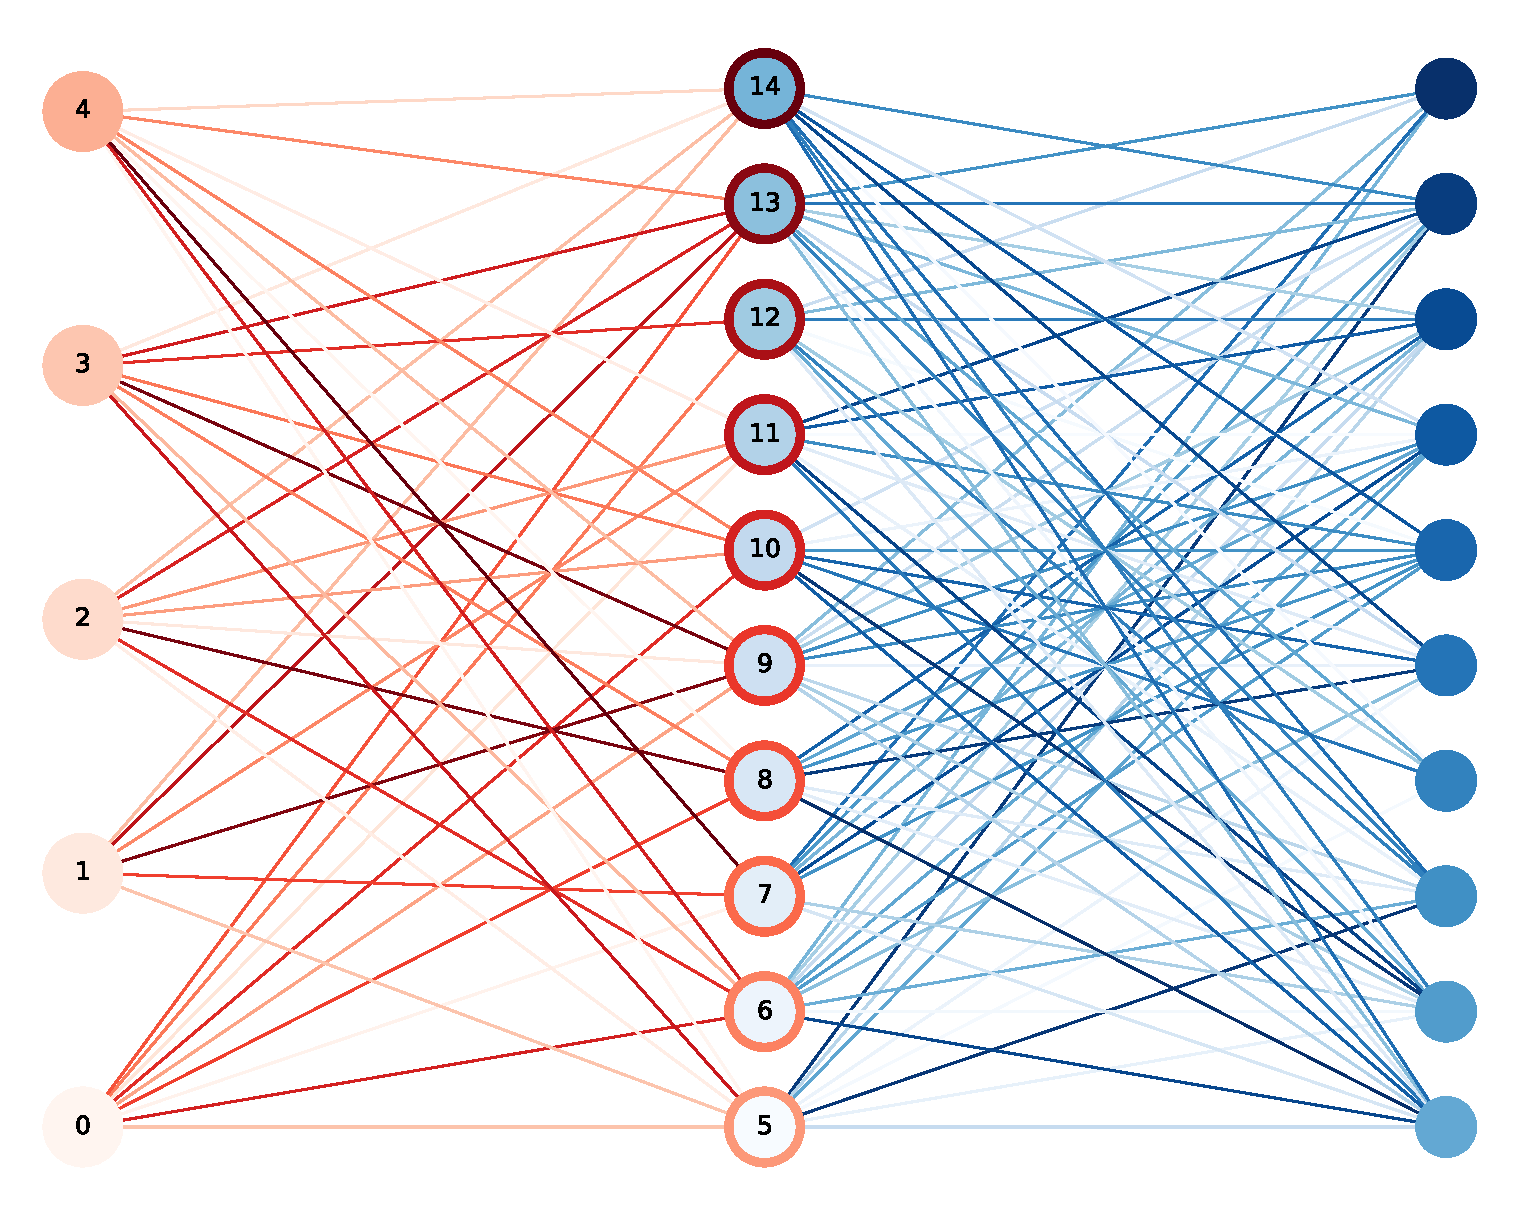
\includegraphics[width=0.45\textwidth]{FigureRobhoot.pdf}
  %\caption{
  {\small {\bf Figure 3: Robhoot in Digital Ecosystems}: {\bf Left
      column}: {\bf $\mathcal{ROBHOOT}$ v.1.0} representing the
    research cycle as nodes from number 0 to 4: Data integration (0),
    Complexity Reduction (1), Inference (2), Validation (3), and
    Visualization(4)). {\bf Central column}: Nodes representing the
    research cycle in the left column are connected to open-source
    software in the digital ecosystem. Connections with node number 0
    in the left column can, for example, represent the ETLs
    open-source software interactions required to generate the {\bf
      Universal ETLs} module. The same meaning applies to the
    different nodes of the left column. {\bf Right column}: Each node
    represents a report meaning there is a reporting gradient
    generated by the connections to the open-source software from
    where each report is generated only using a subset of the research
    layers and open-source software.}
%\end{figure*}


%\section{How to contribute to Robhoot}

%\section{The Robhoot roadmap}
%The following is a first version of the roadmap, the backbone from
%where a more detailed FET-EU proposal will be generated.

\begin{figure*}[ht]
  %\centering
  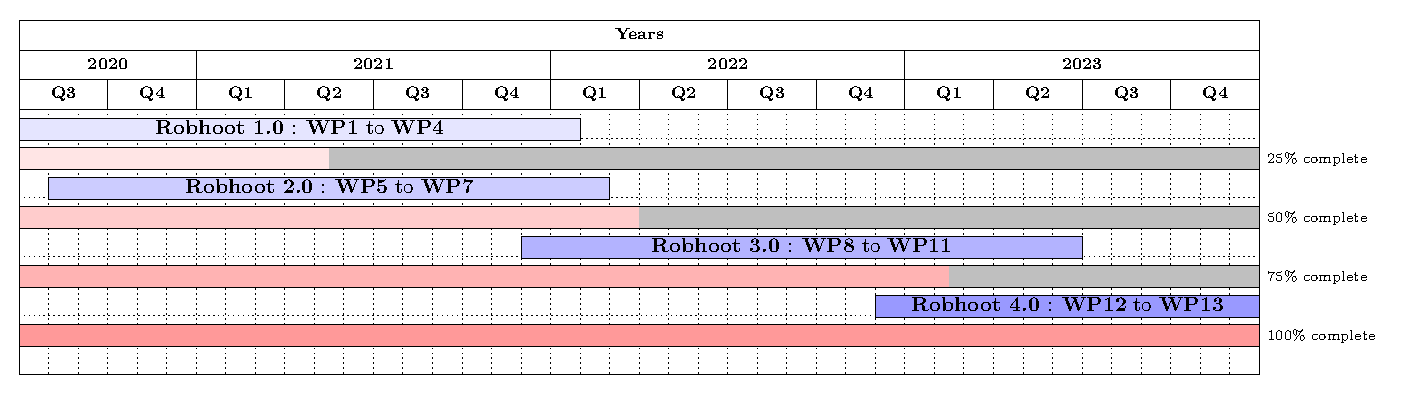
\includegraphics[width=1\textwidth]{GanttChartWhitePaper.pdf}
  %\caption{
  {\small {\bf Figure 4: Roadmap}: {\bf $\mathcal{ROBHOOT}$ v.1.0}
    working packages {\bf WP1} to {\bf WP4} will take care of the
    integration of {\bf Universal ETLs}, {\bf Bayesian Space Models},
    {\bf Animation Space}, and {\bf Reporting} to automate fully the
    research cycle (Figure 2a). {\bf $\mathcal{ROBHOOT}$ v.2.0} {\bf
      WP5} to {\bf WP8} will deploy knowledge graphs (KGs) into a
    fully traceable research cycle (Figure 2b). {\bf
      $\mathcal{ROBHOOT}$ v.3.0} {\bf WP9} to {\bf WP12} will explore
    deep learning networks to sample KGs populations to gain
    understanding of the robustness of the patterns in the data under
    distinct research paths (Figure 2c). {\bf $\mathcal{ROBHOOT}$
      v.4.0} {\bf WP13} to {\bf WP16} will deploy KGs populations into
    a decentralized network of mutually trusting/untrusting peers with
    every peer maintaining the population of the KGs.}
\end{figure*}


%\newpage
\section{Conclusion}
Science and technology ecosystems are in need of accounting for the
uncertainties, reproducibility and immutability related to the
complexity of the research process (Table 1). Such needs are not just
for a specific stage of the research cycle, but from data acquisition
and integration to automated reporting generation because
knowledge-inspired societies and decentralized governance will demand
full research cycle transparency to solve complex social,
environmental and technological problems. Reducing knowledge-gaps at
global scales in knowledge-inspired societies bring many challenges to
our research proposal because obtaining robust knowledge from
integrating many layers of the research cycle, each containing its own
set of methods and uncertainties, can generate divergent, fragile and
contradictory outcomes.

We will develop a flexible and adaptive research method focusing step
by step in increasing levels of complexity (i.e., from {\bf
  $\mathcal{ROBHOOT}$} v.1.0 to v.4.0, Figure 4). Our motivation will
be to provide a first open-access proof of concept of how the
technology works: we will automate reproducible research paths ({\bf
  $\mathcal{ROBHOOT}$} v.1.0) to sample the KGs ({\bf
  $\mathcal{ROBHOOT}$} v.2.0) contrasting deep learning algorithms to
estimate the uncertainty of the ruled-based inference obtained by
fitting predictions to simulated data ({\bf $\mathcal{ROBHOOT}$}
v.3.0). Accounting for the uncertainties of each of the research
stages when sampling the KGs comes from the many distinct paths within
and across the layers in the research cycle (Figure 2a). {\bf
  $\mathcal{ROBHOOT}$} v.4.0 will test a variety of consensus
algorithms to explore the degree of security, decentralization and
scalability of the ledger knowledge network using the generated
population of KGs.

Despite our focus will be bias towards the algorithmic robustness
during the four stages of development, we will implement a
domain-specific case study, a ``Biodiversity, Global Change and
Sustainability Research'', to test the robustness of the rule-based
inference obtained by fitting the KGs to empirical patterns. The high
risk associated to robustly automate the full research cycle for
producing immutable open knowledge will be buffered to a great extend
because the existing digital ecosystem of highly reliable open-source
software tools (Figure 3).

%----------------------------------------------------------------------------------------
%	BIBLIOGRAPHY
%----------------------------------------------------------------------------------------

%\printbibliography[title={Bibliography}] % Print the bibliography, section title in curly brackets

%\newpage
\bibliographystyle{unsrtnat}
%\bibliographystyle{tree.bst}
\bibliography{Robhoot.bib}

%----------------------------------------------------------------------------------------

\end{document}

\hspace{-0.2 in}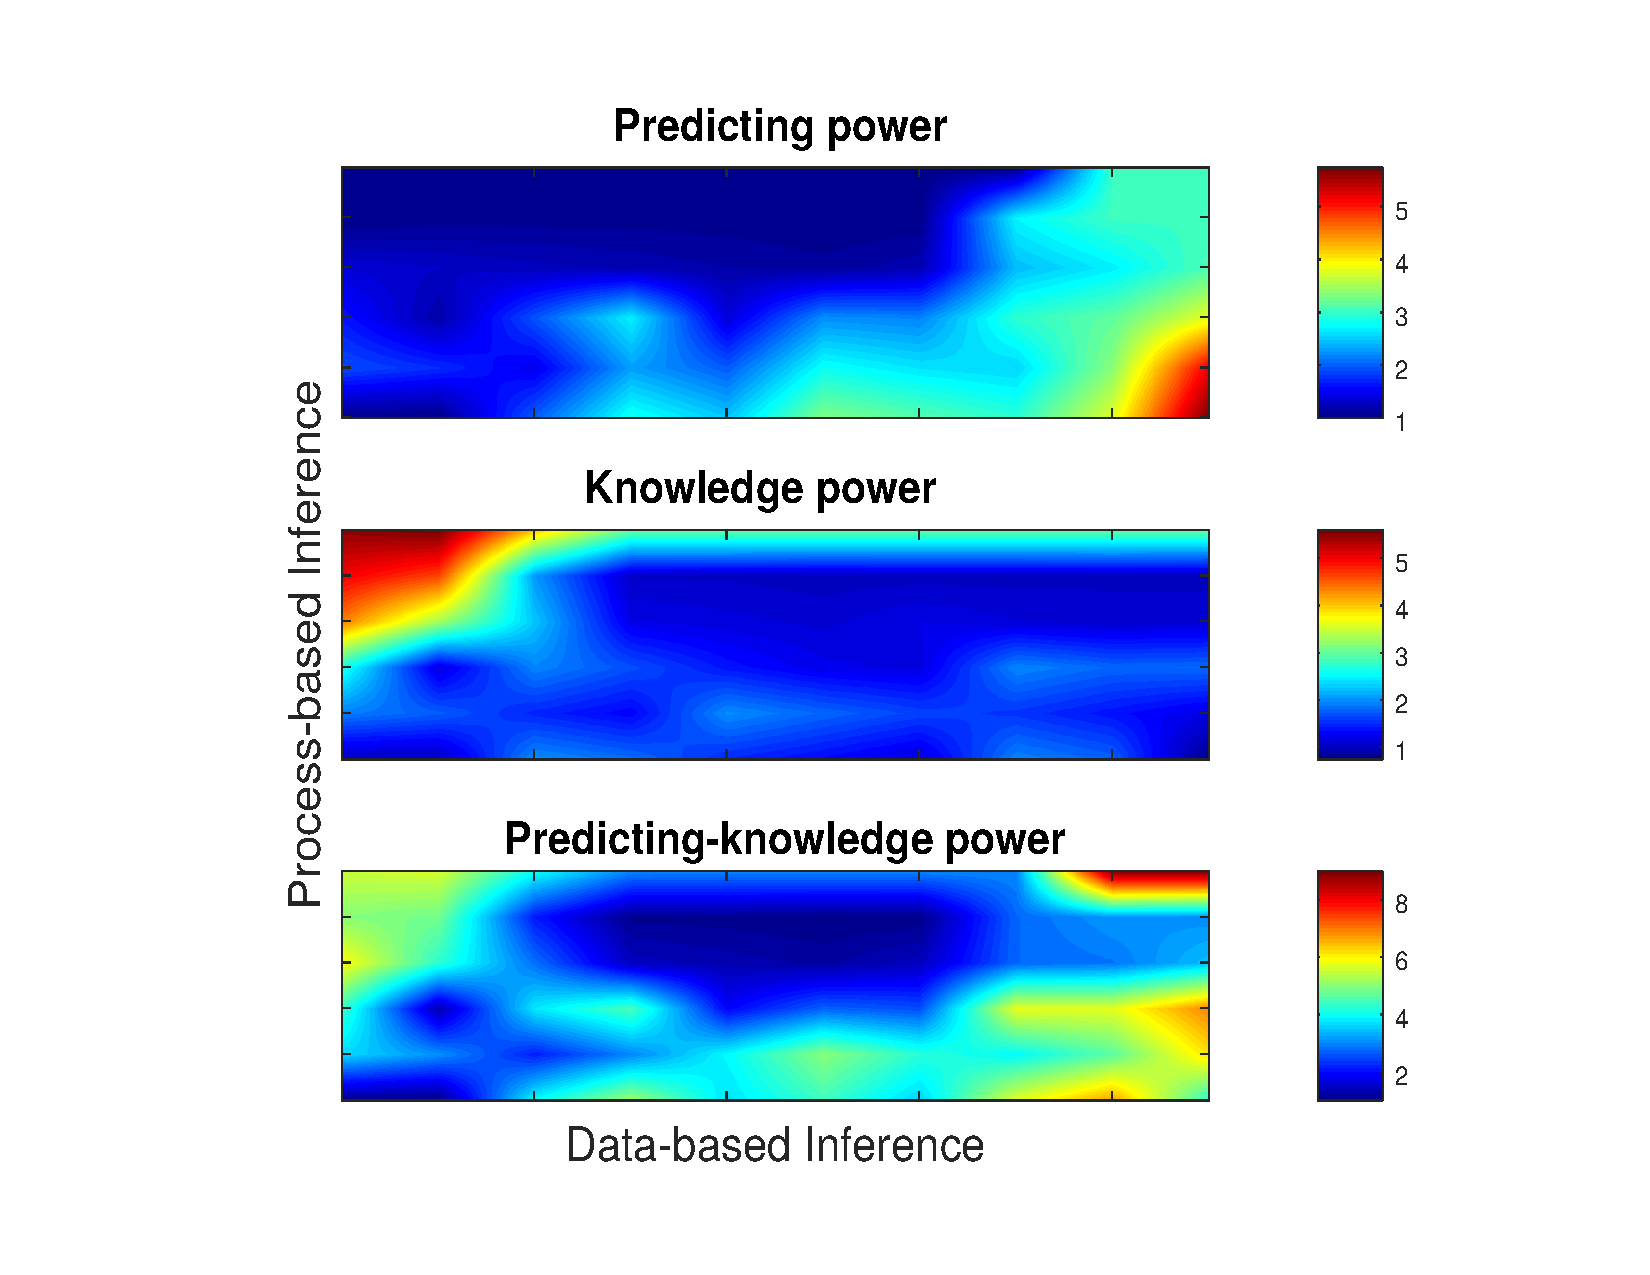
\includegraphics[width=0.52\textwidth]{Figure3.pdf}
{\small {\bf Figure 1: Prediction power (top), understanding (middle),
    and prediction-understanding power maps (bottom)}. x-axis
  represents data-based inference (i.e., gradient of AI methods from
  low (left) to high (right) predictive power). y-axis represents
  process-based inference (i.e., gradient of process-based methods
  from low (bottom left) to high (top left) understanding power). The
  gradient of predicting power map (top) shows a hot spot red area in
  the bottom right highlighting the region where AI methods best
  predict the empirical data. The gradient of understanding power map
  (middle) shows a red hot spot in the top left highlighting the
  region where the best mechanistic understanding occur. The
  predicting-understanding power map (bottom) shows the sum of the two
  previous maps highlighting a red hot spot where the best synthesis
  research joining predicting and understanding power of the empirical
  data might occur. The first research goal of this proposal aims to
  build an automated research platform to maximize the predicting and
  understanding power highlighted in the red hot spot of the
  predicting-understanding power map (bottom).}
